\subsection{Sensing Subsystem}
\label{sec:sensing_subsystem}
The sensing subsystem is an infrared spectrometer that uses two photodiodes as detectors, a diffraction grating as a spectral separator, an array of LEDs to illuminate the target area, and optics to collect, collimate, and focus the beam. In order to determine the component positions and interaction, each component will have to be addressed.
\begin{figure}[H]
    \caption{Sensing subsystem block diagram}
    \centering
    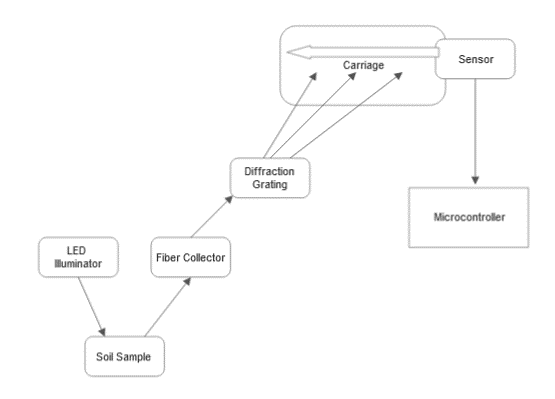
\includegraphics[width=0.75\textwidth]{images/OpticsBlockDiagram.png}
\end{figure}


\paragraph{Overview} The system will determine what automation is needed to optimize the gardening environment using a Near Infrared Optical Spectrometer. The spectrometer will probe the soil with a broad band light source, exciting electromagnetic waves in the weak bonds of the material. These waves will be collimated into a fiber optic cable and transmitted into a closed chamber. The beam will be transmitted onto the surface of a diffraction grating, which will separate wavelengths spatially. A focusing lens will position the separated spectrum on a surface several inches away. Then Visible and Near Infrared optical sensors will be scanned across the surface. At every position, the system microcontroller will record the sensor positions and amplitudes. The data will determine what actions the system will take, whether mechanically or via messaging.

\begin{figure}[H]
    \caption{Spectrometer Ray illustration}
    \centering
    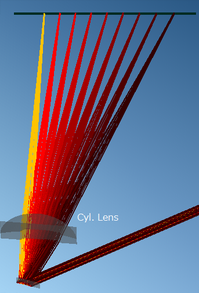
\includegraphics[width=0.25\textwidth]{images/YuanCaoSpectrometer.png}
\end{figure}


\paragraph{Electromagnetic Analysis} Soil is a heterogeneous combination of organic and inorganic substances, and the balance of soil nutrients contributes directly to the quality of the garden environment. Each substance contributes to the total radiative emission of the soil, so by measuring the traces in a sample with unknown quantities and comparing it to traces from a sample with known quantities, the nutrients can be estimated. Soil Carbon content, Moisture Content, Phosphorous, and pH can all be detected within the 400nm to 1700nm range (reference).

\paragraph{Light Source} In order to ensure sufficient signal strength, the soil will have to be excited with light. The spectrum of interest is from 400nm to 1700nm, however, not all data points will be necessary for the system decision matrix. This initially suggested the use of LED lights as a cheap, low power solution, but the number, target wavelengths, and spectral widths of LEDs created several challenges. Broad band Super Luminescent Diodes dramatically reduce the complexity of the problem, but they are an emerging technology with high material cost, placing even the cheapest devices orders of magnitude outside of the project budget. Thankfully, the desired effect can be achieved with a tungsten lamp. Tungsten is a material which emits a broad range of frequencies, covering the spectrum of interest and then some.

\begin{figure}[H]
    \caption{Spectral Output of a Tungsten Lamp}
    \centering
    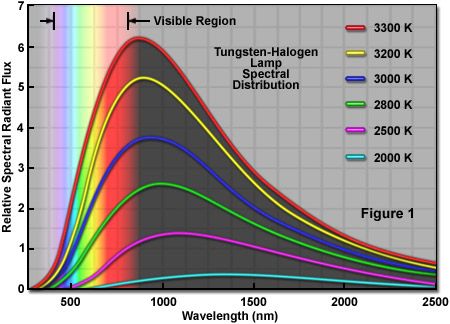
\includegraphics[width=0.75\textwidth]{images/TungstenLamp.jpg}
\end{figure}

\paragraph{Soil Conditions} The optical signal emitted by the soil will be weak, so it is essential that the spectrometer is influenced as much as possible by the content of the soil and as little as possible by the topology of the surface. A well-mixed, smoothly flattened, gently compressed soil sample provides the best conditions for constructing a spectrograph. If there are ridges or depressions along the sample, too much or too little optical signal will pass into the spectrometer, creating an apparent signal strength for wavelengths that is not representative of the soil emission. There are several ways to control these conditions. One is to require the user to retrieve a sample for each scan and deposit it into a spectrometer bay. Another is to require the user to flatten the soil with a spatula or other implement and position the scanner input near the soil. These reduce ease of use, which is a target for the project. Another issue is that the position of the signal input and the tungsten light source relative to the soil sample will have to be consistent to avoid signal error, for the same reasons as above. In (reference) study, this issue was resolved by building a transparent block with slots to hold the light source and the input beam. Their design is represented below, showing the block attached at the rear of a plow chisel for clearing soil while scanning. We will solve the problem of soil topology and light position the same way, by mounting the light source and input fiber in a block of some transparent material like acrylic.

\begin{figure}[H]
    \caption{Fiber Position in Soil Drill}
    \centering
    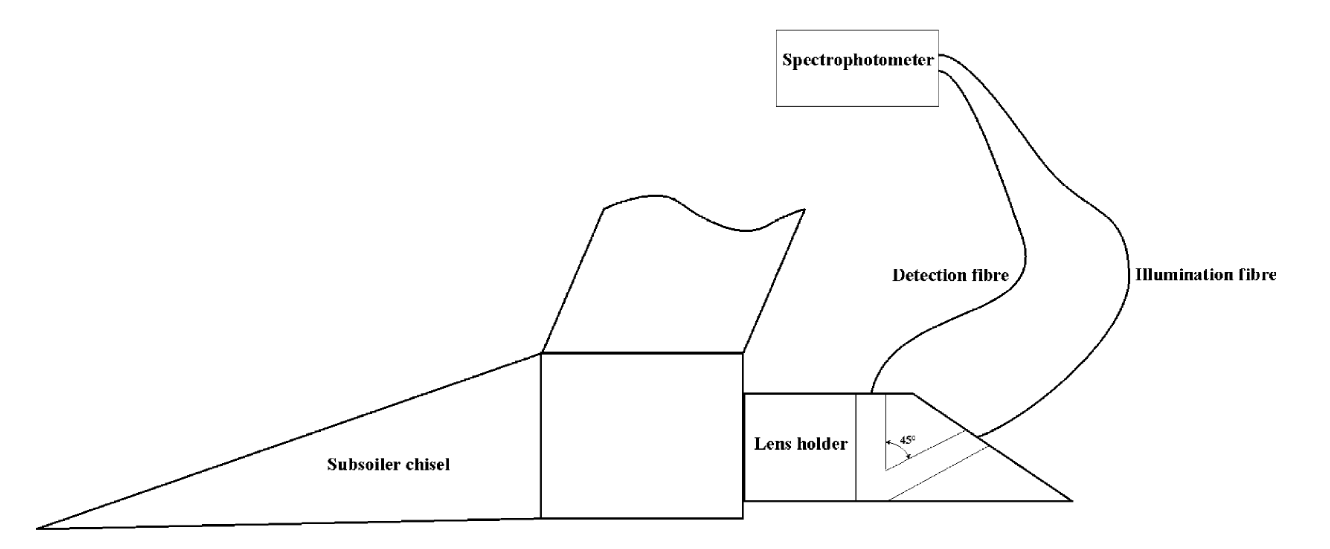
\includegraphics[width=0.75\textwidth]{images/Acrylic Block Fiber positioner.png}
\end{figure}

\paragraph{Fiber Optics} Fiber optic cables are a standard input for spectrometer devices since they allow nearly unlimited flexibility for the position and orientation of the target area relative to the device. The basic ray trace for a lens coupling light into a fiber is shown below. Fiber cores face some basic limitations when it comes to coupling. The maximum possible coupling efficiency can be achieved by pressing the optical surface of the fiber core up against a light source with equal random output in every direction (reference). If the fiber is moved some distance away from the source, less light will impede on the core-air interface. If the core diameter is increased, this will increase the light incident on the core. Light moving in random directions will also strike the fiber core at various angles, however, not all angles of incidence will couple into the fiber. Only rays within the numerical aperture of the fiber will be accepted. This is why installing large lenses at the end of the fiber does not increase the maximum possible amount of light that can be coupled. The maximum angle is determined by the fiber, rather than the collimator.

\begin{figure}[H]
    \caption{Coupling a diffuse light into a fiber}
    \centering
    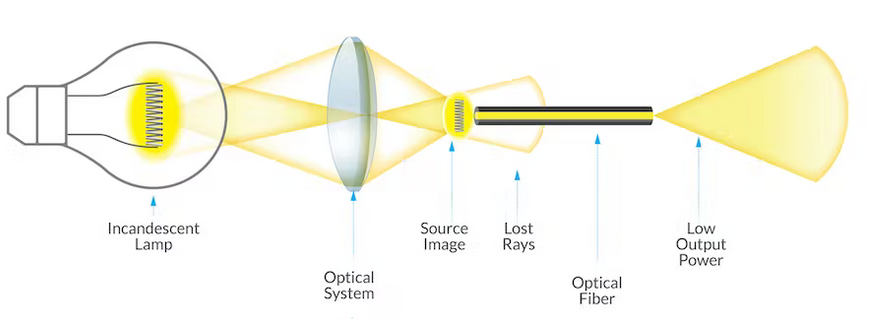
\includegraphics[width=0.75\textwidth]{images/CouplingDiffuseLighttoFiber.png}
\end{figure}

This project involves a large diffuse source, the illumined soil. The Fiber collimator will be attached to the fiber cable via their SMA connectors, then the collimator will be set in an acrylic block so that it rests 8.06mm above the soil. The block will also have a slot for the Light source to illuminate the soil at an angle, similar to the arrangement of the source and sensor in a computer mouse above a mousepad.
The signal will travel through the fiber and up into the spectrometer housing, where the other connector of the cable will be mounted in place. Another collimator will take the output beam and collimate it so that it propagates through free space into the housing. The collimator has an output beam diameter of 1.7mm. This planar wavefront will strike the diffraction grating.

\paragraph{Diffraction Grating} The reflective diffraction grating is a glass mirror with a thin layer of metal deposited on the surface. 1200 lines per millimeter are scored out of the metal horizontally. When a planar wavefront hits the surface of the grating, it reflects off. The confinement of the wave on the surface of the material induces a change of direction proportional to the frequency of the beam, separate from the direction of reflection, equal to the angle of incidence from normal. In order to direct the diffracted beam away from the incoming beam, the grating will be placed at an angle of 45 degrees. This changes the angle of incidence, and determines the angular range of the system. To increase the working range of the grating, the lines scored into it have been blazed at an angle so that light approaching the surface from angle will strike the scored metal at zero degrees from normal. The angular spread of the system will range from the lower angular wavelengths around 400nm up to 1700nm and beyond. 
\begin{figure}[H]
    \caption{Grating Angular Calculation}
    \centering
    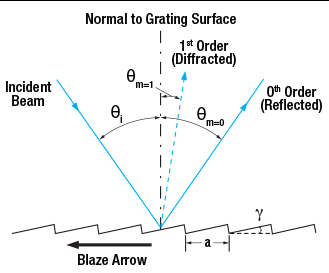
\includegraphics[width=0.4\textwidth]{images/ThorlabsGratingTutorial.png}
\end{figure}


\begin{equation}
    a[sin(\theta m)+sin(\theta i)] = m\lambda
\end{equation}

\begin{figure}[H]
    \caption{Diffraction angle calculation}
    \centering
    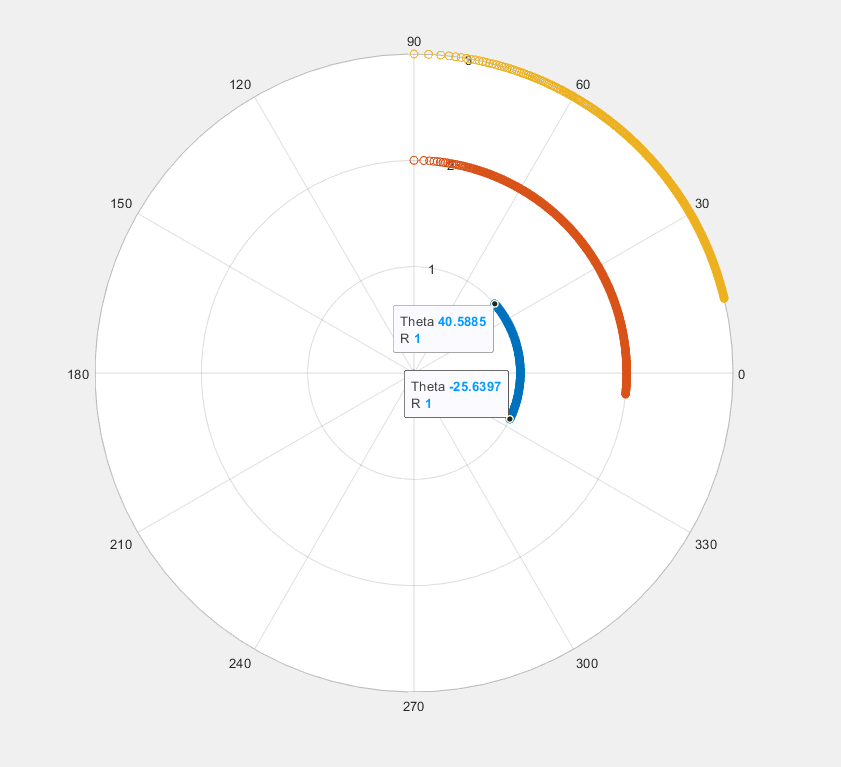
\includegraphics[width=0.75\textwidth]{images/DiffractionAngleCalculator.png}
\end{figure}

The beam coming out of the fiber will have a nonzero width. When the 1.7mm diameter beam hits the surface of the grating, since the grating is at 45 degrees from the beam, light will be propagating from an area with a diameter larger than 1.7mm.


This means the spread of the diffracted light will be 38 degrees in and 21 degrees out from both the near edge and the far edge of the collimated beam on the surface of the grating. In order to capture this light and sort it so that the scanner can proceed linearly through each band, a focusing optic will be needed that covers the full angular range.

\begin{figure}[H]
    \caption{Ray Trace of Diffraction Grating}
    \centering
    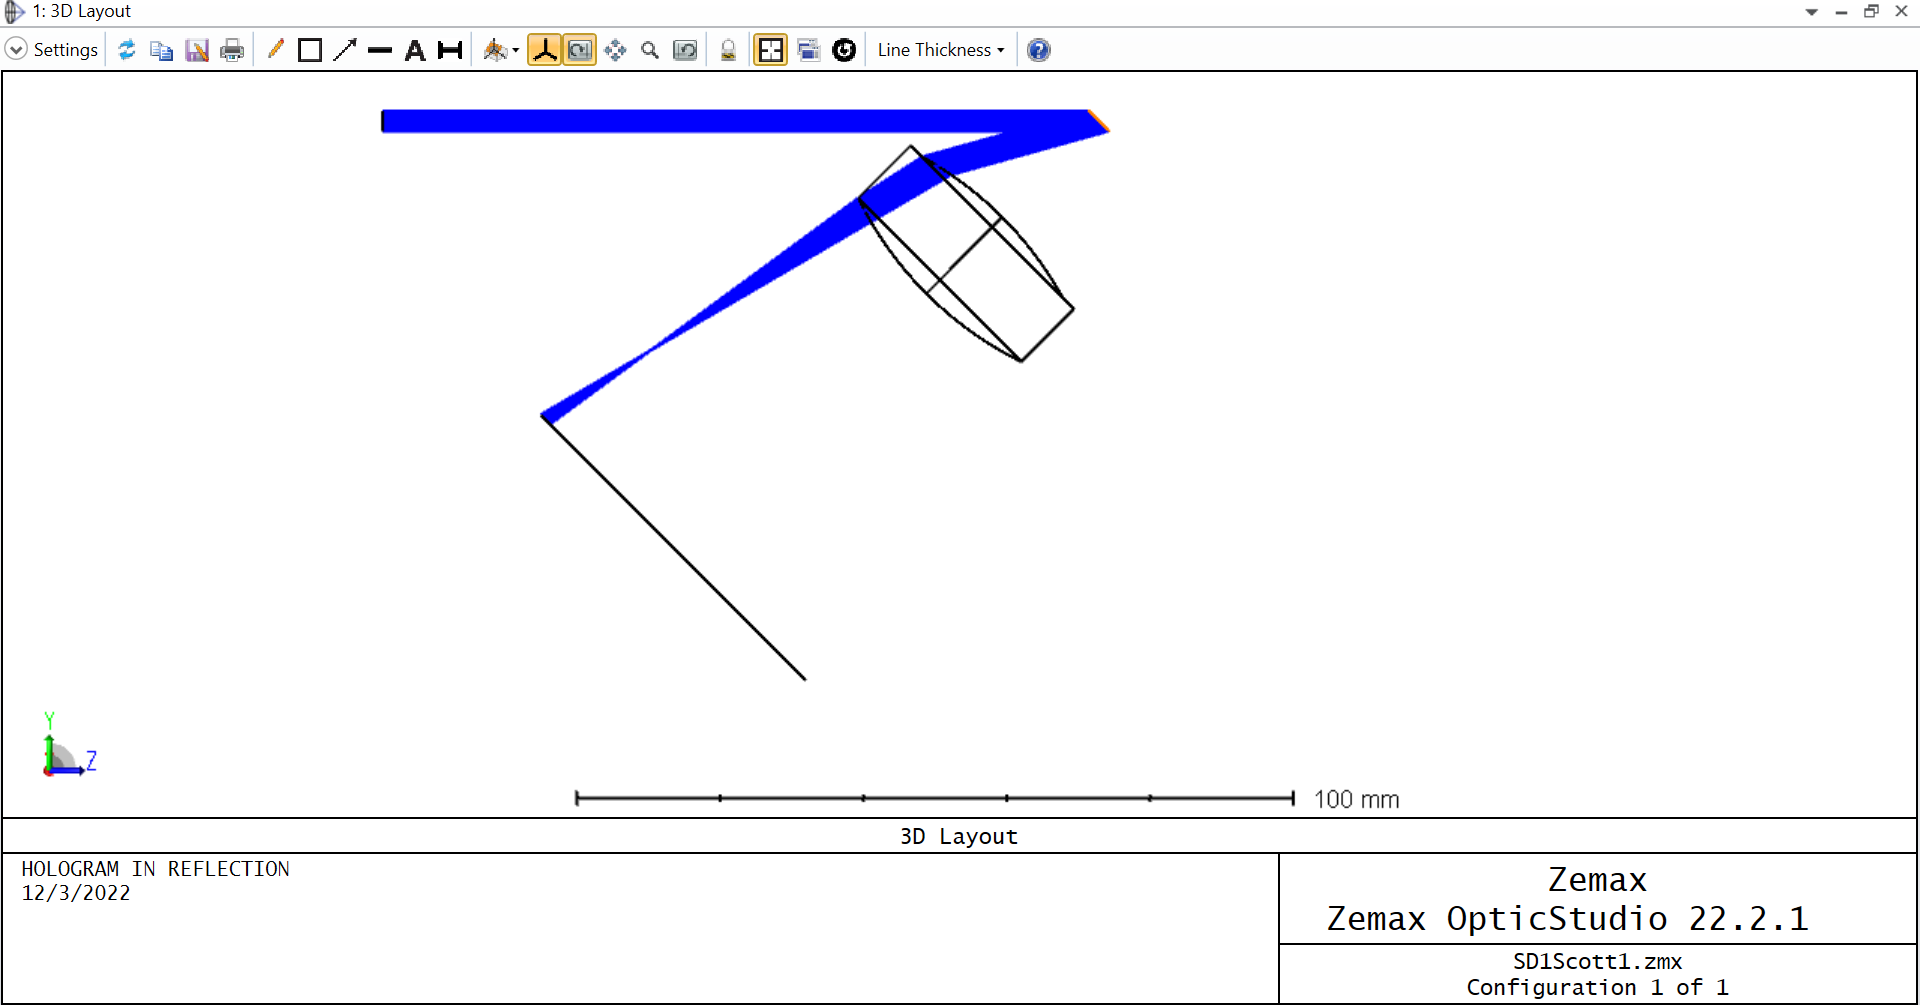
\includegraphics[width=0.75\textwidth]{images/Zemax Ray Trace.png}
\end{figure}

\paragraph{Focusing Lens} The diffraction grating will diverge the beam away from the sensor surface. This divergence can be corrected with a lens, focusing the divergent light to a spot the size of the sensor or smaller. There are two lens designs that could work, spherical and cylindrical. Spherical lenses are polished with a radius of curvature along both the horizontal and vertical axes. The advantage of a spherical lens is that they are generally cheaper to manufacture and available in a wider variety of sizes and shapes. The spot size of a circular beam passing through a spherical lens will be determined by the distance from the focal length, and the spot will be circular. Cylindrical lenses are cut with a radius of curvature along the horizontal axis, but flat along the vertical axis. A circular beam that passes through a cylindrical lens will be focused to the shape of an ellipse, allowing for more vertical flexibility of alignment. Plano-cylindrical lenses offer another advantage, they have a flat bottom, perpendicular to their planar back. This means they can be stood upright and pressed against a flat surface, dramatically reducing the complexity of the optical mount required to hold them in place. Unfortunately, cylindrical lenses are a specialty part with a smaller market, due to their elliptical focusing pattern, and this turned out to make them cost prohibitive for the project. The dimensions and position of the lens are determined by two things, the angular range of the spatially separated beams coming off the reflective diffraction plate, and the width of the scanning region. The lens is also constrained by the angle and width of the input beam, as shown in the ray trace below. If the width of the lens comes within a few wavelengths of the beam approaching the diffraction plate, the beam will diffract around its edge.

\begin{figure}[H]
    \caption{Basic Ray Trace}
    \centering
    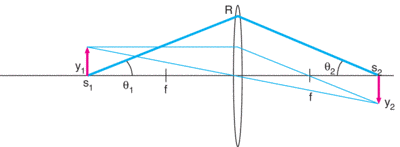
\includegraphics[width=0.75\textwidth]{images/BasicRayTrace.png}
\end{figure}

\begin{figure}[H]
    \caption{Sensor Ray Trace}
    \centering
    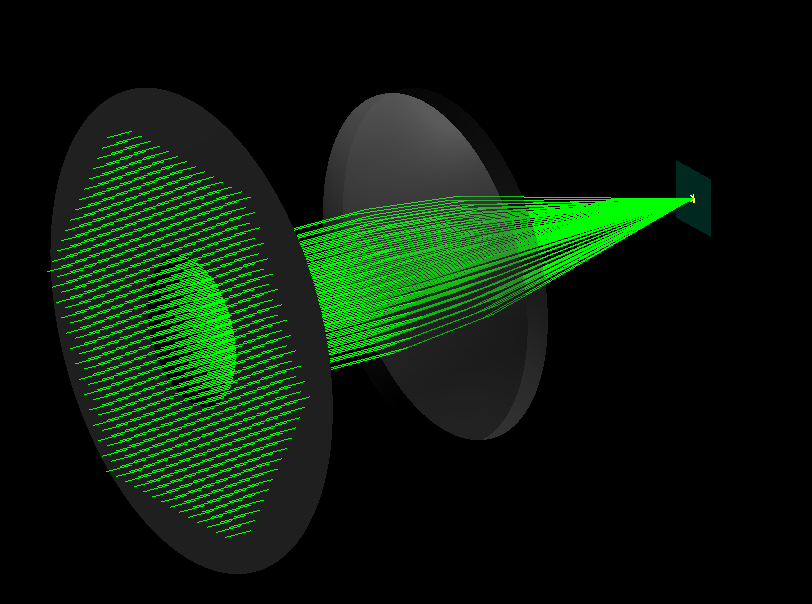
\includegraphics[width=0.5\textwidth]{images/ColimatedBeam.png}
\end{figure}


\paragraph{Circuitry} The Photodiode works by converting a small portion of the incident light into electrical current across the face of the semiconductor. There are three components to the sensing circuitry. First, there is a voltage divider. This voltage divider provides a clean and stable $3.3V/2$ to the anode of the photodiode. From there the team will use a 1M$\Omega$ resistor to and an op-amp to convert current to voltage to get a current resolution of 1 $\mu$A/V.
\begin{figure}[H]
    \caption{Sensing Schematic}
    \centering
    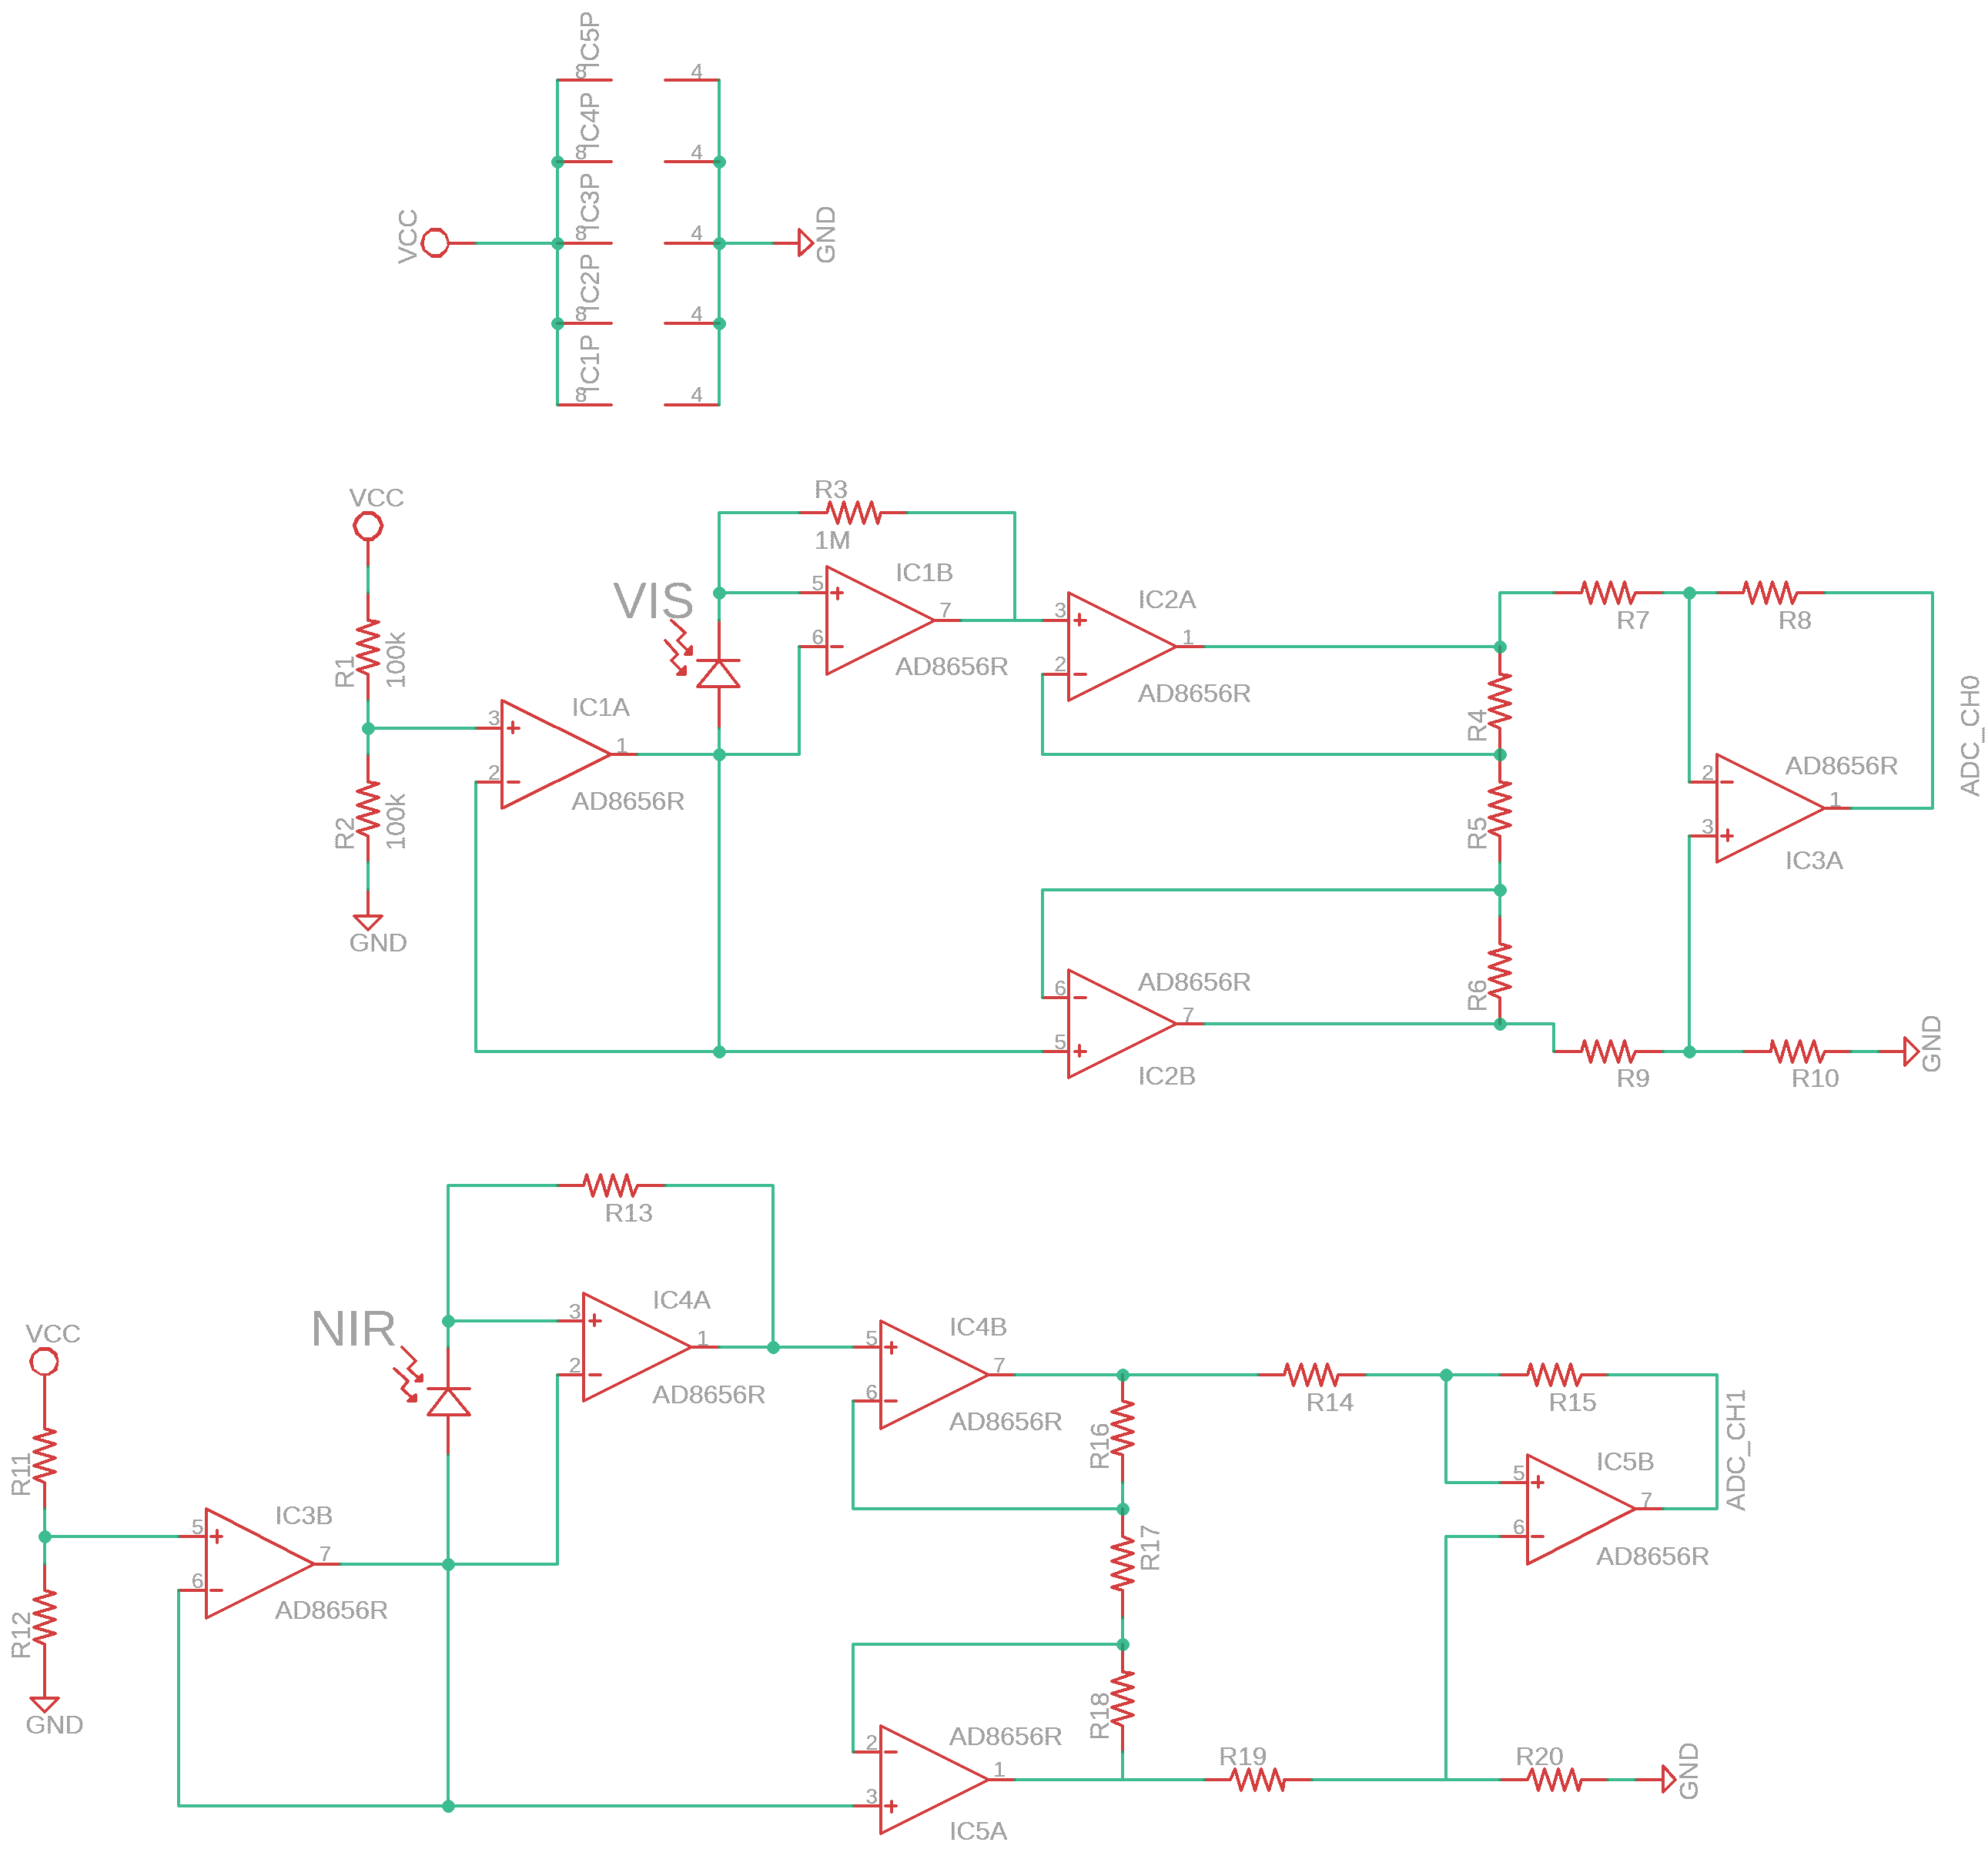
\includegraphics[width=.8\textwidth]{images/sensor-schematic.png}
    \label{fig:sensor-schem}
\end{figure}

\begin{figure}[H]
    \caption{Soil Spectrograph}
    \centering
    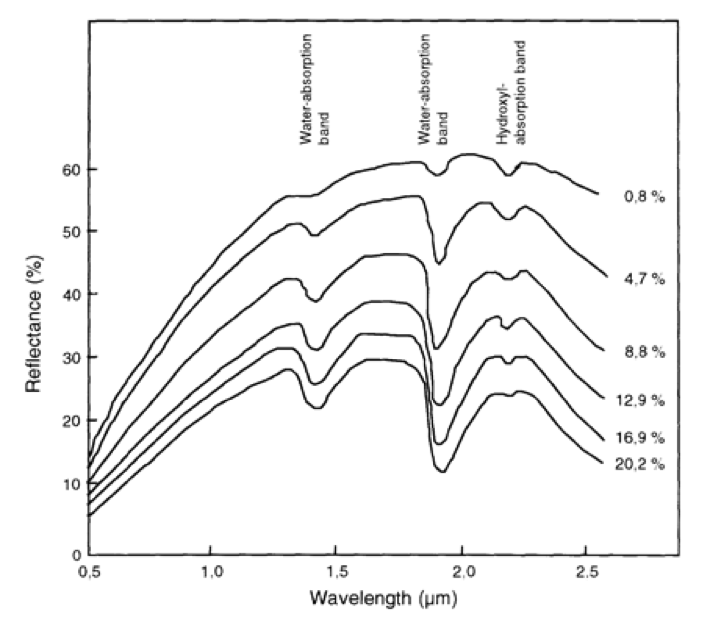
\includegraphics[width=0.75\textwidth]{images/GenericSoilSpectra.png}
\end{figure}

